\chapter{Introduction}
\label{introduction}


\section{General Introduction}
Humans have used body characteristics such as face, voice or even gait to recognize each other for thousands of years. In the mid-19th century, Alphonse Bertillon (chief of the criminal identification division of the police department in Paris, France) developed and then practised the idea of using body measurements to identify criminals. In the late 19th century, the idea of Bertillon lost popularity due to the far more practical discovery of the distinctiveness of human fingerprints (\cite{jain_biometrics}). 

Nowadays, biometrics have advanced to the point that it is no surprise if criminals are imprisoned because their fingerprints were found in the crime scene. However, other biometric methods are not as known as fingerprints and for certain people it is something that can only be found in science fiction movies. Their doubts are not unfounded, biometrics have long been used in science fiction movies to portray futuristic worlds of advanced technology. From retina scans to voice identification and facial recognition, these technologies have been seen on the big screen for more than 50 years (\cite{biometrics_in_scifi}). 

Nonetheless, as we can see in \cite{iphonex_and_other_uses}, face recognition is already being used around the world to examine, investigate, and monitor. There it is explained how in the United States, more than half of all American adults are in a face recognition database that can be used for criminal investigations, simply because they have a driver’s license. In the UK, face recognition was also used at an annual West Indian cultural festival to identify revelers in real-time. 

Although biometrics, and therefore face recognition, emerged from its extensive use in law enforcement to identify criminals, it is being increasingly used today to establish person recognition in a large number of civilian applications (\cite{jain_biometrics}), such as the recently released FaceID for the new iPhone model that identify the face of the owner to unlock the phone. 

The technology around face recognition has advanced following diverse paths, being neural networks the most recent and successful. Within neural networks, there is one particular type of deep, feedforward network that was much easier to train and generalized much better than networks with full connectivity between adjacent layers. This was the \gls{cnn}. It has achieved many practical successes during the period when neural networks were out of favour and it has recently been widely adopted by the computer-vision community (\cite{lecun2015deep}). 

With the advent of several open source libraries, face recognition is now possible and available for everyone. Among this motley group of open source libraries, we find Tensorflow, originally developed by the Google Brain team for the purposes of conducting \gls{ml} and deep neural networks research (\cite{tensorflow_main_website}). Despite the fact that before TensorFlow there were plenty of \gls{ml} libraries that offered great functionality and were reasonably well documented (e.g. \cite{theano_main_site}, \cite{caffe_main_site}), this library has become very popular in the last years thanks to its powerful yet easily readable API, written in Python. 

These such libraries would not be possible without the previous work done in the fields of \gls{ml}, \gls{ai} and face recognition by researchers like Yann LeCun, Yoshua Bengio or Geoffrey Hinton (\cite{rumelhart1985learning}, \cite{lecun1995convolutional}, \cite{lecun1998efficient}, \cite{lecun1998gradient}, \cite{bengio2009learning}, \cite{krizhevsky2012deep}, \cite{lecun2015deep}), and it will be further discussed in the following sections.

In this report we will explain the development of an application that we have called \textit{Intelligent Asissistant}. It is based in one of the currently most advanced implementations of face recognition: FaceNet (\cite{facenet_article}), heavily inspired by the previous OpenFace (\cite{amos2016openface}). Here we will use Tensorflow to re-train a kind of \gls{cnn} named \textit{Resnet Inception v1} from one of the models that FaceNet has left available in their Github website (\cite{facenet_github}).

The objective of the \textit{Intelligent Assistant} is to help the students of the University of Limerick in their first days around the University. This help consists in showing them which is the next class that they will have in the day and the path to the classroom. Face recognition is used here to confirm the identity of a student and be able to search the timetable of such student. Other identification approaches were also available, but as a biometric system, face recognition allow students to be identified by "who they are", rather than "what they possess" (e.g. student ID card) or "what they remember" (e.g. password), which may be things not very clear in the first caotic days in the University. 

The timetable information can be publicly accessed, in the website \textit{timetable.ul.ie}, so applying a technique known as web \gls{scraping}, the student's timetable is obtained and then analysed in order to find their next class. The path to the next class will be shown as a Google Map image, using the Static Google Map API (\cite{google_maps_static}). The face recognition process is preceded by a face \textit{detection} process, that will crop the face out of the image, removing the background and making easier the identification.

Architecturally, the \textit{Intelligent Assistant} is divided in a laptop, which will run the server that actually perform the different tasks of the assistant, and a small, low-cost and basic computer called Raspberry Pi, which will run the \gls{gui} used to interact with the application and will communicate with the server to obtain the needed information. The whole application is written in Python, allowing us to use the Tensorflow library and to learn this popular language, which, as the topics of \gls{ai} and \gls{ml}, was not previously taught in the study program. 

%\section{Technologies Used}	
%
%	\subsection{Why TensorFlow?}
%	We have talked about TensorFlow as it would be the only library available, but there are many more, some of them even written also in Pyhton . That said, why choose it instead other deep learning library? First, TensorFlow is one of the newest libraries at the moment of writing for deep learning in Python and we want this project to deal with a current issue. And second, this library has two APIs (\cite{tensorflow_main_website}): a high level API (MNIST), which makes it accessible for everyone and it will be easy to start with; and a low level API (Deep MNIST), which can provide a more advanced control for the final development of the project.
%
%	\subsection{Why Raspberry Pi?}
%	TensorFlow still needs a computer with a certain computing power, which also means that it will have a considerable size. In order to provide mobility to the assistant, a client-server architecture is going to be used. In the server side is where face recognition and high computing requirement tasks are actually going to be executed, while the client side will act as the interface of the system. 
%
%	As the client side will not require much computing power, Raspberry Pi becomes an option. With the size of a credit card, Raspberry Pi is a low-cost and barebones computer capable to work as a traditional desktop tower. Many versions of this board have been released, but for this project we have chosen the Raspberry Pi 3 Model B.
%
%	\begin{figure}[ht]
%		\centering
%		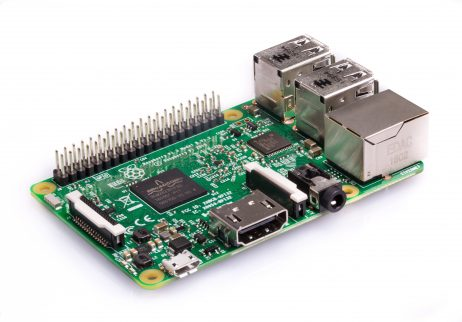
\includegraphics{raspberry-pi-3-b.jpg}
%		\caption{Raspberry Pi 3, model B}
%	\end{figure}
%
%	\subsection{Why Python?}
%	The reasons that made Python the language chosen for this project were many. First, it is the language that Tensorflow uses to express the model of the network, so it was necessary to use it at least for the face recognition module of the project. Second, Python has become a widely used language because (\cite{why_python}):
%
%	\begin{itemize}
%		\item Proven language. Python is used by many important companies, such as Dropbox, Google or Amazon. 
%		\item Fast prototypes. Python's dynamic nature and simple syntax make it perfect for prototyping, preventing us from worrying about the actual implementation and helping to focus on data and algorithms, which the main task of machine learning.
%		\item For everyone. Many data scientist and engineers have a background in maths and statistics, but they may not have any experience in programming. Python's simplicity and readability, as it is said to have a math-like syntax, make it easier to pick up.
%		\item Mature Data Science Ecosystem. There is a great collection of math and data science for Python, incremented by new libraries that are built on top of the older ones (but controlled by the solid Python's packaging). 
%	\end{itemize}
%
%	Finally, the last reason is personal. During the last years in my home University, I heard many times how important Python was and how popular it was becoming. However, the modules from my study program never used this language for their assignments, so I never had the opportunity to learn it in an academic environment. Because of that, I decided to use Python in all aspects of this project in order to learn how to work with it.  

\section{Objectives}
The objectives of this project are many and can be divided in personal and technical. The first and more important personal one is to learn about the fields of Computer Science with which I never experimented before. In my home University (Carlos III of Madrid), I chose the computer architecture specialization in my third year. This means that my knowledge about \gls{ai} and \gls{ml} was almost not existent, as it was taught in the other specializations. 

The situation with the Python language at the beginning of the year was similar, even when it is a well known language and has become very popular in the last years. The modules from my study program never used this language for the assignments, so I never had the opportunity to learn it in an academic environment. Because of that, when my coordinator explained me that for the Tensorflow library I would need to use Python, I decided to use it. Not only in the interaction with the library, but also in the server communication and the application \gls{gui}.

On the other hand, among the technical objectives of this project we can find:
\begin{itemize}
	\item Create a tool called \textit{Intelligent Assistant} to help the students of the University of Limerick to find their next class.
	\item Use Python for the development of this tool.
	\item Divide the system in a client-server communication in order to achieve a light-weight application in the client side.
	\item Use the microframework Flask (never used before either), also written in Python, to create the server.
	\item Use a Raspberry Pi in the client side to act as interface with the students.
	\item Design a graphical user interface that allows to use all the features of the application.
	\item Perform face recognition using the Tensorflow library to identify the students.
	\item Show in the final stage a map with the path from the current position to the location of the next class.
\end{itemize}

\section{Motivation}
This \gls{fyp} was motivated for many reasons that started with the idea of doing it abroad. In my third year I decided to do my fourth and final year of the degree as an Erasmus student, but it was too late to be included in the Erasmus lists of that year. The only option to be able to go on Erasmus was to finish my degree one year later, so I splitted the modules of the fourth year in two groups with the idea of doing the first half of the modules in my fourth year in Spain, and the other half abroad. 

Althought it was forced by the circumstances, I do not regret the fact of doing my \gls{fyp} abroad. It gave me the opportunity to improve my academic writting in English by doing this document, reaching a total of X pages and becoming the longest document I have ever written in English. I must apologise about this fact, because English is not my mother tongue and, even when I have spent much time looking for grammatical errors, there may still be some that I could not detect.

Another motivation of this project, already mentioned in the previous section, was to learn about topics that my degree in Spain did not cover in its study program. The decission I took in my third year of choosing the \textit{computer architecture} specialization closed me the doors to learn about \gls{ai} and \gls{ml}, so this project was the perfect occasion to expand my knowledge on such topics. Besides, other related (e.g. face detection, face recognition) and not related (e.g. Python, web \gls{scraping}, \gls{gui} design) issues that were never treated before, were also included in the project in order to learn more about them. 

\section{Structure of the Document}
This present document is divided in:

\begin{itemize}
	\item Glossary of Terms and Acronyms. List of definitions of the terms and acronyms that have been used in this report and that may result confusing for the reader. Every term and acronym used in the text is linked its definition here.
	\item Introduction. This section, in which we are currently in, includes a little background about biometrics and \gls{ml}, along with a brief explanation of the project and the reasons that motivated its realization.  
	\item Research. In this section, the state of the art of the different fields with which this project is related (i.e. machine learning, neural networks, face detection and face recognition) and some of the technologies used, are widely explained, referencing the books and papers from where the factual information actually comes from. 
	\item Design and Implementation. The complete development process of the \textit{Intelligent Assistant} application can be found here.
	\item Empirical Studies. A total of two empirical studies are included in this section, treating the effectiveness of the approaches used in the project for the face detection (i.e. Viola-Jones Haar cascades) and the face recognition (i.e. \glspl{cnn}).
	\item Discussion and Conclussion.
	\item Appendices. 
	\begin{itemize}
		\item Appendix A. Set of icons used in the \gls{gui} of the application.
		\item Appendix B. Actual captures of the final version of the \gls{gui} of the application.
	\end{itemize}
\end{itemize}



